\documentclass{fairmeta}

\usepackage{amsmath}
\usepackage{enumerate} 
\usepackage{algorithm}
\usepackage{algpseudocode}
\usepackage{amsfonts}
\usepackage{amsthm}
\usepackage{newtxtt}
\usepackage{algorithm}
\usepackage{cleveref}
\usepackage{diagbox} 
\usepackage{colortbl}
\usepackage{nicematrix}
\usepackage{subcaption}


\usepackage[frozencache,cachedir=.]{minted}

\usepackage{tcolorbox}
\usepackage[framemethod=tikz]{mdframed}
\usepackage{amssymb}
\usepackage{xspace}
\usepackage{wrapfig}
\usepackage{adjustbox}
\usepackage{tabularx}
\usepackage{booktabs}
\usepackage{mathtools}


\usepackage{tikz}
\usetikzlibrary{positioning, calc}
\usetikzlibrary{decorations.pathmorphing}

\usepackage{silence}
\makeatletter
\patchcmd{\wrong@fontshape}{\@gobbletwo}{}{}{}
\makeatother
\WarningFilter{latexfont}{Font shape}
\WarningFilter{latexfont}{Some font}


\input{math_commands}
\newcommand{\highlight}[1]{{\color{metablue} \textbf{#1}}}
\newmdenv[backgroundcolor=metabg, roundcorner=5pt, skipabove=7pt, linewidth=0pt, innertopmargin=4pt]{myframe}
\newcommand{ \metatriangleright }{ {\color{metablue} \blacktriangleright} }
\renewcommand{\eqref}[1]{\labelcref{#1}}


\numberwithin{equation}{section} 
\setcounter{tocdepth}{2} %


\tcbuselibrary{minted}

\usemintedstyle{colorful}

\setminted[python]{
  linenos,
  breaklines,
  fontsize=\footnotesize,
  xleftmargin=2em
}

\definecolor{light}{RGB}{125, 125, 125}

\crefname{tcb@cnt@pbox}{code}{code}
\Crefname{tcb@cnt@pbox}{Code}{Code}
\crefname{assumption}{assumption}{assumption}
\Crefname{assumption}{Assumption}{Assumptions}

\newtcolorbox[auto counter]{pbox}[2][]{
  colback=white,
  title=Code~\thetcbcounter: #2,
  #1,fonttitle=\sffamily,
  fontupper=\sffamily,
  arc=10pt,
  colframe=metabg,
  coltitle=metafg,
  colbacktitle=metabg,
  toptitle=0.25cm,
  bottomtitle=0.125cm
}


\title{Persistent Segment Trees\\
\large{CS 4501: Advanced Algorithms and Implementation, Spring 2025\\}
}

\author[1]{Riley Immel}
\author[1]{Windsor Antal}
\author[1]{Brandon Yang}


\affiliation[1]{University of Virginia}



\date{\today}
\metadata[Code]{\url{https://github.com/rileyimmel/persistentSegTreesProject}}

\begin{document}

\maketitle

% \tableofcontents
% \clearpage
% \newpage

\section{Introduction}\label{section:intro}

Recall when we first introduced the concept of a \textbf{Segment Tree} in class. The Segment Tree is a data structure that allows us to efficiently query and update ranges of values in an array. Formally, given a list of integers $A = \{a_1, a_2, \dots, a_n\}$, and a function $f(l, r)$ that operates on a continuous subsegment $A[l \dots r]$, the Segment Tree provides two key operations. The first operation is a range query, which calculates $f(l, r) = f(a_l, \dots, a_r)$ for any given indices $l$ and $r$ ($l \le r$) in $O(\log n)$ time. The second operation is a point update, which updates the value of an element $a_i$ at any index $i$ in $O(\log n)$ time. Overall, we can build a Segment Tree in $O(n)$ time, and it uses $O(n)$ space.

Suppose we want to maintain a Segment Tree for a list of integers $A = \{a_1, a_2, \dots, a_n\}$, but we also want to keep track of the history of updates made to the array. In other words, we want to be able to query the value of $a_i$ at \textit{any} point in time, not just the current value. This is where the concept of a Persistent Segment Tree comes into play.

Formally, a \textbf{Persistent Segment Tree} is a data structure that extends the Segment Tree to support \textit{versioned}  range queries and updates, allowing access to any past state of the array efficiently. Given an initial array $A = \{a_1, a_2, \dots, a_n\}$, the Persistent Segment Tree maintains a sequence of immutable versions $\mathcal{T}_0, \mathcal{T}_1, \dots, \mathcal{T}_k$, where each version $\mathcal{T}_i$ corresponds to the state of the Segment Tree after $i$ updates. This is achieved via \textit{path copying}, where only $O(\log n)$ nodes are copied for each update. The Persistent Segment Tree supports the following operations:

\begin{itemize}
    \item \textbf{Build:} Constructs the initial tree $\mathcal{T}_0$ from the array $A$ in $O(n)$ time and space.
    \item \textbf{Persistent Update:} Given a version $\mathcal{T}_i$ and an index $p \in [1, n]$, and a new value $v$, creates a new version $\mathcal{T}_{i+1}$ such that $a_p$ is replaced with $v$ in $\mathcal{T}_{i+1}$, while all other values remain unchanged. This operation takes $O(\log n)$ time and $O(\log n)$ space.
    \item \textbf{Range Query:} Given a version $\mathcal{T}_i$ and indices $l, r \in [1, n]$, computes $f(l, r)$ in $O(\log n)$ time. This operation does not require any additional space.
    \item \textbf{Version Access:} Allows retrieval and independent querying of any previous version $\mathcal{T}_j $ for $j \le i$. This operation takes $O(1)$ time and space.
\end{itemize}

\section{Background}\label{section:background}

\subsection{Segment Tree Recap}

A Segment Tree is a binary tree structure built over an array $A$. Each node in the tree corresponds to a specific range $[l, r]$ of indices in the original array and typically stores the precomputed value of the function $f$ over the subsegment $A[l \ldots r]$. We define the Segment Tree $\mathcal{T}$ recursively as follows:

\begin{itemize}
    \item \textbf{Base Case (Leaf Node):}
          If $l = r$, then the node labeled as $a[l \dots r]$ stores:
          \[
              \text{sum} = A[l]
          \]

    \item \textbf{Recursive Case (Internal Node):}
          If $l < r$, let $m = \left\lfloor \frac{l + r}{2} \right\rfloor$. Then the node labeled as $a[l \dots r]$ stores:
          \[
              \text{sum} = f\left(\text{left child sum},\ \text{right child sum}\right)
          \]
\end{itemize}

The function $f$ determines how two child nodes are combined. For example, in the sum Segment Tree shown in Figure~\ref{fig:segment_tree_example}, $f(x, y) = x + y$.


\begin{figure}[H]
    \centering
    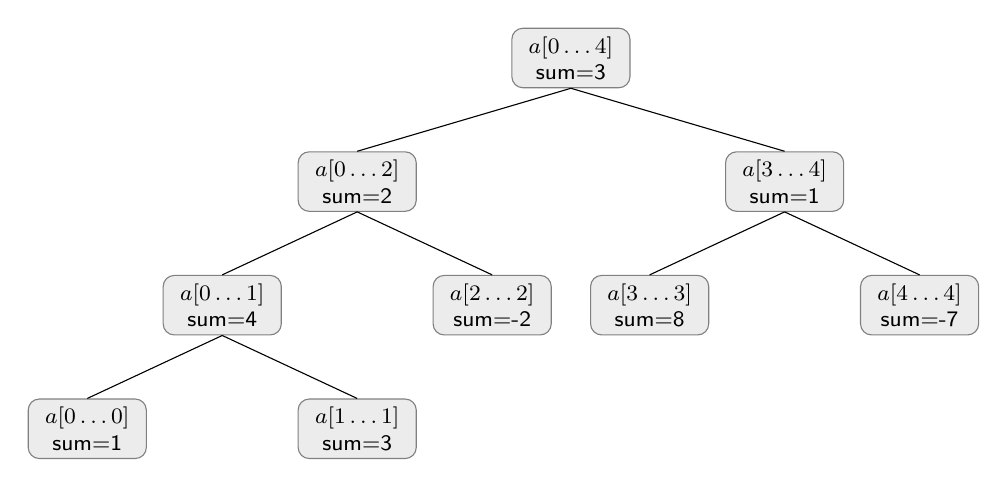
\begin{tikzpicture}[
            node distance=0.8cm and 0.2cm,
            treenode/.style = {align=center, inner sep=3pt, text centered,
                    font=\sffamily\footnotesize, rectangle, rounded corners, draw=gray, fill=gray!15, minimum width=1.5cm}
        ]
        \node (root) [treenode] {$a[0 \dots 4]$\\ sum=3};
        \node (l)    [treenode, below left = of root, xshift=-10mm] {$a[0 \dots 2]$\\ sum=2};
        \node (r)    [treenode, below right= of root, xshift=10mm] {$a[3 \dots 4]$\\ sum=1};
        \node (ll)   [treenode, below left = of l] {$a[0 \dots 1]$\\ sum=4};
        \node (lr)   [treenode, below right= of l] {$a[2 \dots 2]$\\ sum=-2};
        \node (rl)   [treenode, below left = of r] {$a[3 \dots 3]$\\ sum=8};
        \node (rr)   [treenode, below right= of r] {$a[4 \dots 4]$\\ sum=-7};
        \node (lll)  [treenode, below left = of ll] {$a[0 \dots 0]$\\ sum=1};
        \node (llr)  [treenode, below right= of ll] {$a[1 \dots 1]$\\ sum=3};

        \draw (root.south) -- (l.north);
        \draw (root.south) -- (r.north);
        \draw (l.south)    -- (ll.north);
        \draw (l.south)    -- (lr.north);
        \draw (r.south)    -- (rl.north);
        \draw (r.south)    -- (rr.north);
        \draw (ll.south)   -- (lll.north);
        \draw (ll.south)   -- (llr.north);
    \end{tikzpicture}
    \caption{Segment Tree for $A = [1, 3, -2, 8, -7]$ with sum aggregation. Each node stores the range $[l, r]$ and the corresponding aggregated value, which is the sum of the values in that range. The root node represents the entire array, while the leaf nodes represent individual elements. The internal nodes represent the sum of their respective child nodes.}
    \label{fig:segment_tree_example}
\end{figure}

\section{Approach}\label{section:approach}

The key idea behind the Persistent Segment Tree is that we want to preserve all previous versions of the Segment Tree while still allowing efficient updates and queries. A naïve way to do this would be to copy the entire tree every time we perform an update, but this would lead to an inefficient $O(n)$ time and space cost per update. Instead, we use a technique called \textbf{path copying}, which ensures that only $O(\log n)$ new nodes are created per update, while the rest of the structure is shared.

Each time we perform a point update on the Persistent Segment Tree, we create a new version of the tree that reflects the update, while keeping all previous versions intact. Rather than constructing a completely new tree, we reuse all parts of the existing tree that remain unchanged. The only nodes that need to be recreated are those that lie on the path from the root to the updated leaf. This is done by creating a new node for the the updated value and recursively copying the necessary nodes along the path to the root. The rest of the tree remains unchanged, allowing us to maintain a history of all previous versions.

Each version of the Segment Tree is identified by a unique root node. These root nodes are stored externally, so that querying any historical version simply requires passing the corresponding root into a standard query function. All queries and updates remain $O(\log n)$, just like in a regular Segment Tree.

\begin{figure}[H]
    \centering
    \begin{tikzpicture}[
            node distance=0.8cm and 0.2cm,
            newnode/.style = {treenode, draw=metablue, fill=metablue!10},
            newedge/.style = {draw=metablue},
            sharededge/.style = {draw=metablue, dashed},
            treenode/.style = {align=center, inner sep=3pt, text centered,
                    font=\sffamily\footnotesize, rectangle, rounded corners, draw=gray, fill=gray!15, minimum width=1.5cm}
        ]
        \node (root0) [treenode] {$a[0 \dots 4]$\\ sum=3};
        \node (l)    [treenode, below left = of root0, xshift=-10mm] {$a[0 \dots 2]$\\ sum=2};
        \node (r)    [treenode, below right= of root0, xshift=10mm] {$a[3 \dots 4]$\\ sum=1};
        \node (ll)   [treenode, below left = of l] {$a[0 \dots 1]$\\ sum=4};
        \node (lr)   [treenode, below right= of l] {$a[2 \dots 2]$\\ sum=-2};
        \node (rl)   [treenode, below left = of r] {$a[3 \dots 3]$\\ sum=8};
        \node (rr)   [treenode, below right= of r] {$a[4 \dots 4]$\\ sum=-7};
        \node (lll)  [treenode, below left = of ll] {$a[0 \dots 0]$\\ sum=1};
        \node (llr)  [treenode, below right= of ll] {$a[1 \dots 1]$\\ sum=3};

        \draw (root.south) -- (l.north);
        \draw (root.south) -- (r.north);
        \draw (l.south)    -- (ll.north);
        \draw (l.south)    -- (lr.north);
        \draw (r.south)    -- (rl.north);
        \draw (r.south)    -- (rr.north);
        \draw (ll.south)   -- (lll.north);
        \draw (ll.south)   -- (llr.north);

        \draw[->, thick, shorten <=10pt, shorten >=10pt]
        ([xshift=10pt]root0.south) -- ([xshift=10pt]l.north);
        \draw[->, thick, shorten <=10pt, shorten >=10pt]
        ([xshift=10pt]l.south) -- ([xshift=10pt]ll.north);
        \draw[->, thick, shorten <=10pt, shorten >=10pt]
        ([xshift=10pt]ll.south) -- ([xshift=10pt]llr.north);



        \node[right=0.1cm of root0, anchor=west] {$\mathcal{T}_0$};
        \node[right=0.1cm of root0, yshift=1cm, anchor=west] {$\verb|update|(1, 5)$};
        \node (root1) [newnode, left=2mm of root0] {$a'[0 \dots 4]$\\ sum=5};
        \node (l1)    [newnode, below left = of root1, xshift=-10mm] {$a'[0 \dots 2]$\\ sum=4};
        \node (l1l)  [newnode, below left = of l1] {$a'[0 \dots 1]$\\ sum=6};
        \node (l1lr) [newnode, below right= of l1l] {$a'[1 \dots 1]$\\ sum=5};
        \node[left=0.1cm of root1, anchor=east] {$\mathcal{T}_1$};

        \draw[->, thick, blue, shorten <=10pt, shorten >=10pt]
        ([xshift=-10pt]l1lr.north) -- ([xshift=-10pt]l1l.south);
        \draw[->, thick, blue, shorten <=10pt, shorten >=10pt]
        ([xshift=-10pt]l1l.north) -- ([xshift=-10pt]l1.south);
        \draw[->, thick, blue, shorten <=10pt, shorten >=10pt]
        ([xshift=-10pt]l1.north) -- ([xshift=-10pt]root1.south);


        \draw[newedge] (root1.south) -- (l1.north);
        \draw[newedge] (l1.south)    -- (l1l.north);
        \draw[newedge] (l1l.south)    -- (l1lr.north);

        \draw[sharededge] (root1.east) -- (root0.west);
        \draw[sharededge] (l1.east) -- (l.west);
        \draw[sharededge] (l1l.east) -- (ll.west);
        \draw[sharededge] (l1lr.east) -- (llr.west);


    \end{tikzpicture}
    \caption{\textbf{Path Copying Illustration:} Given Segment Tree $\mathcal{T}_0$ for $A = [1, 3, -2, 8, -7]$ with sum aggregation, we perform a persistent update to change the value at index $1$ from $3$ to $5$. This creates a new version $\mathcal{T}_1$ by copying only the nodes along the path from the root to the updated leaf. All other nodes are shared with the original version. Nodes created for $\mathcal{T}_1$ are shown in blue, and shared nodes are connected by dashed edges.}
    \label{fig:pathcopying}
\end{figure}


Figure~\ref{fig:pathcopying} illustrates the path copying mechanism when an update occurs. The tree on the left, $T_0$, represents the original Segment Tree. When an update is applied, a new version $T_1$ is created. Nodes that are not affected by the update (i.e., not on the path to the updated index) are shared between the two versions. Only the nodes along the update path are newly allocated and updated.

This design makes the Persistent Segment Tree a powerful tool for problems that require historical access, undo functionality, or multi-version computations. In the next section, we will describe the detailed recursive implementation of the Persistent Segment Tree, including how versions are stored, how queries are performed, and how updates generate new roots with minimal copying.

\section{Implementation}\label{section:implementation}

Given an array $A = [a_1, a_2, \dots, a_n]$, we first build a standard Segment Tree $\mathcal{T}_0$ in $O(n)$ time. We also need to initialize a list of roots $\mathcal{R} = [\mathcal{T}_0]$ to store the roots of all versions.

\subsection{Persistent Update Algorithm}

Let $\texttt{Node}$ represent a node in the Segment Tree, containing:
\begin{itemize}
    \item \texttt{val}: the aggregate value over the range $[l, r]$,
    \item \texttt{left}, \texttt{right}: pointers to the left and right child nodes.
\end{itemize}

Let $f : V \times V \to V$ be an associative \emph{merge function} (e.g., sum, min, max) used to combine the results from the left and right subtrees.

We define the update procedure $\texttt{update}(\texttt{node},\ l,\ r,\ p,\ v)$, where:
\begin{itemize}
    \item \texttt{node} is the root of the current version,
    \item $[l, r]$ is the range that \texttt{node} covers,
    \item $p$ is the index to update,
    \item $v$ is the new value to assign at index $p$.
\end{itemize}

\vspace{0.5em}
\noindent The function returns a new root node for the updated version. The update is defined recursively as follows:

\begin{itemize}
    \item \textbf{Base Case:} If $l = r = p$, then we have reached the leaf node to be updated. Return a new node:
          \[
              \texttt{Node}(v,\ \texttt{None},\ \texttt{None})
          \]

    \item \textbf{Recursive Case:} Otherwise, let $m = \left\lfloor \frac{l + r}{2} \right\rfloor$.

          \begin{itemize}
              \item If $p \le m$, we update the left subtree:
                    \[
                        \texttt{left} \gets \texttt{update}(\texttt{node.left},\ l,\ m,\ p,\ v), \quad \texttt{right} \gets \texttt{node.right}
                    \]
              \item If $p > m$, we update the right subtree:
                    \[
                        \texttt{left} \gets \texttt{node.left}, \quad \texttt{right} \gets \texttt{update}(\texttt{node.right},\ m+1,\ r,\ p,\ v)
                    \]
          \end{itemize}

          Return a new internal node combining the updated child and the reused child:
          \[
              \texttt{Node}\left(f(\texttt{left.val},\ \texttt{right.val}),\ \texttt{left},\ \texttt{right}\right)
          \]
\end{itemize}

\vspace{0.5em}
\noindent\textbf{Time and Space Complexity:} Each call to $\texttt{update}$ creates $O(\log n)$ new nodes, one per level along the path from the root to the updated leaf. Thus, each update runs in $O(\log n)$ time and uses $O(\log n)$ space.

\subsection{Range Query and Version Access}

To query any version $\mathcal{T}_k$, we simply pass its root into the standard Segment Tree range query function. Since version roots are stored externally, accessing a particular version takes $O(1)$ time, and the query itself runs in $O(\log n)$ time as usual.

\section{Summary of Programming Challenge}

\textbf{Desks of Eternity} is a versioned data structure challenge where students implement a system to track dynamic updates to an array while maintaining full historical access to any prior state. The learning objective is to teach students how to apply persistent data structures—in this case, a persistent segment tree—to support efficient point updates and range queries across multiple versions of data.

The key twist in the assignment is handling not just value updates (replacements), but also \textbf{nontrivial operations like swaps and max-history-based replacements} (``perfect''), while keeping the structure efficiently queryable across versions. This goes beyond basic persistent trees by requiring students to design a strategy to manage \textbf{shared structure with non-monotonic changes}, making it both a data structures and systems design exercise.

\subsection*{Key Ideas for Solving Programming Challenge}

To solve this challenge, students must use a \textbf{persistent segment tree} to store historical versions of evaluation scores, enabling range queries across any pair of versions. The main challenge lies in supporting:
\begin{itemize}
    \item \textbf{Swaps}, which affect two positions and break the naïve one-path update assumption.
    \item \textbf{Perfect replacements}, which require maintaining per-index history of maximums.
\end{itemize}

These challenges require students to reason about how to store auxiliary data (like max-history per index) and adapt standard persistence techniques. The final solution has $O(\log n)$ update and query time per operation, and $O(n + c \log n)$ space for all versions. The problem is rich enough to reinforce key data structure principles without exceeding the capabilities of an upper-level undergraduate student.

\section{Conclusion}

We discuss the implementation of a Persistent Segment Tree, a powerful data structure that allows efficient updates and queries across multiple versions of an array. The key idea is to use path copying to minimize the space and time complexity of updates while maintaining the ability to access any previous version. This design is particularly useful for problems that require historical access or multi-version computations.

We also designed a programming challenge, ``Desks of Eternity,'' to reinforce the concepts of persistent data structures and their applications in real-world scenarios. The challenge requires students to implement a system that tracks dynamic updates to an array while maintaining full historical access to any prior state, using a Persistent Segment Tree.


% \begin{pbox}[label={ex:fm_standalone}]{Standalone Flow Matching code \\ \url{flow_matching/examples/standalone_flow_matching.ipynb}}
%     \inputminted{python}{assets/demo.py}
%     \vspace{0.5cm}
%     \includegraphics[width=\textwidth]{assets/half_moons.png}
% \end{pbox}

\appendix
\newpage

% \section{Python Implementation of Persistent Segment Tree}\label{sec:python_implementation}
% \begin{pbox}[label={ex:euler_method}]{Python Implementation of Persistent Segment Tree}
%     \begin{minted}[linenos, breaklines, mathescape, fontsize=\footnotesize, xleftmargin=2em]{python}
% class Node:
%     def __init__(self, value=0, left=None, right=None):
%         self.value = value
%         self.leftChild = left
%         self.rightChild = right

% class PST:
%     MAX = 100

%     def __init__(self, n):
%         self.n = n
%         self.version = 0
%         self.root = [None] * self.MAX

%     def construct(self, val):
%         self.root[0] = self._construct(val, 0, self.n - 1)

%     def _construct(self, val, l, r):
%         node = Node()
%         if l == r:
%             node.value = val[l] if val else 0
%             node.maximum = val[l] if val else 0
%             return node
%         middle = (l + r) // 2
%         node.leftChild = self._construct(val, l, middle)
%         node.rightChild = self._construct(val, middle + 1, r)
%         node.value = node.leftChild.value + node.rightChild.value
%         return node

%     def _update(self, l, r, prev, idx, new_val):
%         node = Node()
%         if l == r:
%             node.value = new_val
%         else:
%             middle = (l + r) // 2
%             if idx <= middle:
%                 node.leftChild = self._update(l, middle, prev.leftChild, idx, new_val)
%                 node.rightChild = prev.rightChild
%             else:
%                 node.rightChild = self._update(middle + 1, r, prev.rightChild, idx, new_val)
%                 node.leftChild = prev.leftChild
%             node.value = node.leftChild.value + node.rightChild.value
%         return node

%     def _query(self, node, l, r, ql, qr):
%         if l > qr or r < ql:
%             return 0
%         if ql <= l and qr >= r:
%             return node.value
%         middle = (l + r) // 2
%         return self._query(node.leftChild, l, middle, ql, qr) + \
%             self._query(node.rightChild, middle + 1, r, ql, qr)

%     def update(self, idx, val):
%         self.version += 1
%         self.root[self.version] = self._update(0, self.n - 1, self.root[self.version - 1], idx, val)

%     def query(self, query_version, l, r):
%         return self._query(self.root[query_version], 0, self.n - 1, l, r)
% \end{minted}
% \end{pbox}

% \pagebreak

\end{document}
